\section{Metode}
\noindent\textbf{Utstyr}:
\begin{itemize}
    \item Telefon
    \item Telefonholder
    \item Trefot
    \item Vater
\end{itemize}
VARIANT 1:
For målingene ble en trefot brukt for å stabilisere telefonen og sørge for minst mulig bevegelse som kunne påvirke resultatene. Et vater siktet først inn på Nidarosdomen og telefonen ble lagt ved siden av vateret som figur \ref{fig:med_vater} viser. Før alle målingene ble gjort ble programmet Phypox kalibrert ved å snu rundt på mobilen i rundt 30 sekunder. Det ble så gjort tre målinger med tre forskjellige mobiler. Dette gjentok seg tre ganger.

Så ble vateret siktet inn på tyholttårnet på samme måte som målingene på Nidarosdomen ble gjennmført. Denne gangen ble mobilen slåt..
Målingene ble gjort rett utenfor hovedbygningen til NTNU i starten av broen på veien "Øvre Alle" slik at det var både mulig å se toppen av Nidarosdomen og tyholttårnet på samme sted.  \newline


VARIANT 2:
En trefot ble brukt som plattform for telefonene, hvor telefonene ble plassert i en teleofonholder. For å gi riktig retning på telefonene, ble det plassert ett vatert langsmed telefonholderen. Vateret ble så brukt som siktemiddel slik at telefonholderen, og dermed telefonen lå i retning som det objektet som ble siktet på \ref{fig:med_vater}. Deretter ble plattformen justert slik at den var horisontal ved hjelp av et vater. 
Før hver måling ble telefonene «kalibrert» ved å spinne de rundt. Deretter ble telefonene plassert i telefonholderen og ble liggende der en stund. Dataene ble så eksportert. Samme prosess ble gjennomført med retning mot Tyholt tårnet og Nidarosdomen. 
Det ble også testen om flymodus og restarting av telefonene ville ha noen effekt. Testen med flymodus ble gjennomført ved at telefonene ble satt i flymodus og dermed satt i telefonholderen. Testen med restarting ble gjennomført ved at telefonene ble restartet og så igjen «kalibrert» før de ble plassert i telefonholderen.
For å finne posisjonen ble phyphox benyttet. Da med «Location» som gir GPS koordinater. Telefonene ble kalibrert ved at de ble beveget noen meter i ulike retninger før selve målingen ble utført i telefonholderen. Målingene ble utført på vestre siden av broen som krysser Eidsvolls gate langs Øvre alle. 
Dataene ble så analysert i Python ved hjelp av teorien beskrevet ovenfor, for å finne gjennomsnittsverdi, median og standardavvik. For å finne vinklene mellom referansesytemet mot Tyholttårnet og Nidarosdomen ble biblioteket geographiclib benyttet.  

 
\begin{figure}
    \centering
    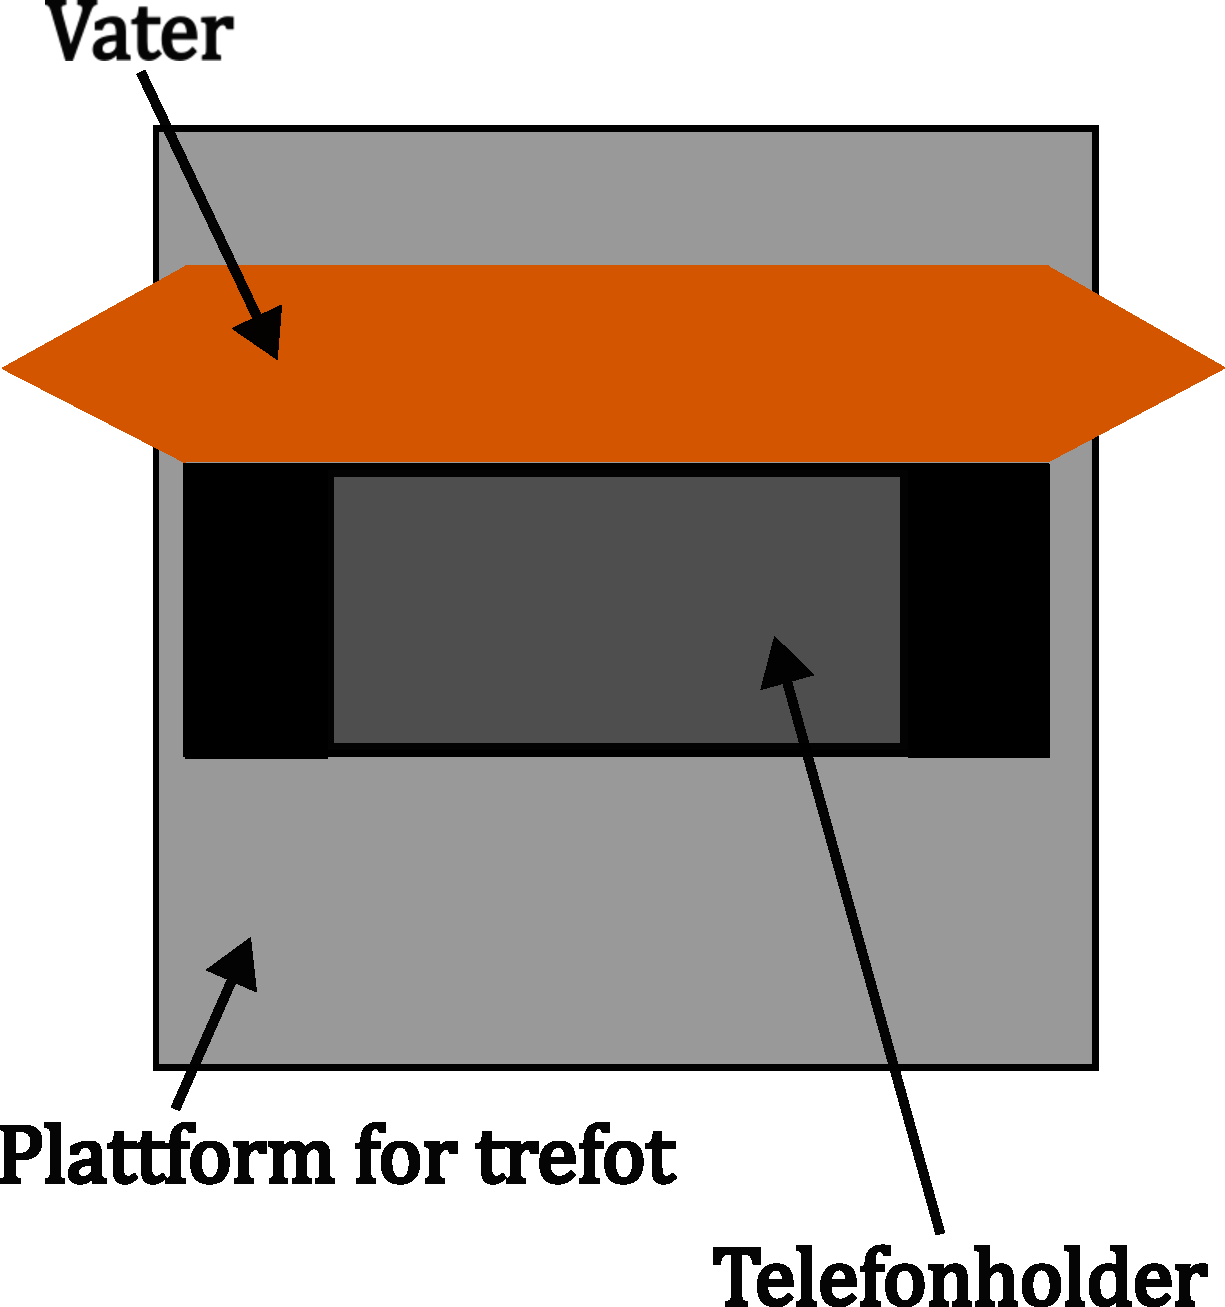
\includegraphics[width=0.45\textwidth]{img/Plattform med vater.pdf}
    \caption{Figuren viser oppsettet under målingene. Et vater ble brukt for å sikte inn på Nidarosdomen og Tyholttårnet og viste i hvilken retning mobilen skulle ligge. 
        }
    \label{fig:med_vater}
\end{figure}